% !TeX root = ../thesis.tex

\chapter{Implementation}
\label{sec:implementation}
We use PointPillars\cite{lang_pointpillars_2019} as the detection model at most Experiments. Cause PointPillars' inference speed is fast and has relative higher precision. After adversarial attacks and defenses apply to victim network. The processing speed will be 2 times or 3 times slower than original one. So the running time of victim model is more important. The code is based on OpenPCDet\cite{openpcdet2020}, We use R40\cite{simonelli_disentangling_2019} as Average Precision(AP) to evaluate different levels of cars. The threshold of IoU for different levels of cars is 0.7.
\section{FGSM}
\subsection{Selection of Epsilons}

\(\epsilon\) is a parameter in FGSM, which determines the extent of perturbation. In our experiment, we choose epsilons ranging from 0.001 to 0.2 to do attacks, and the attack result is in Figure \(\ref{fig:Select Epsilons}\). By observing the curve, we choose the epsilons in each tuning point to take further experiments: 0.01, 0.02, 0.04. 

As the Figure \(\ref{fig:FGSM Comparison}\) shown, we apply 3 different \(\epsilon\) on the point clouds and we could see the changes between original point clouds(OPC) and OPC added perturbation calculated by FGSM with \(\epsilon\) 0.04 is easy to tell. OPC is almost the same as OPC added perturbation by FGSM with \(epsilon\) 0.01. For  

\begin{figure}[htbp]
\centering
\subfigure[OPC]{
\begin{minipage}[t]{0.25\linewidth}
\centering
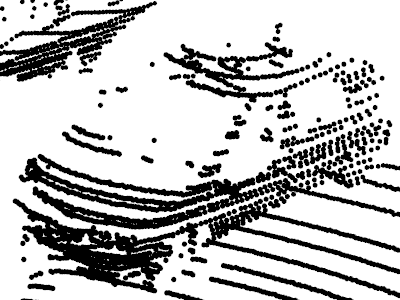
\includegraphics[width=1in]{Graphics/LidarCar0.png}
%\caption{fig1}
\end{minipage}%
}%
\subfigure[FGSM with \(\epsilon\) 0.01]{
\begin{minipage}[t]{0.25\linewidth}
\centering
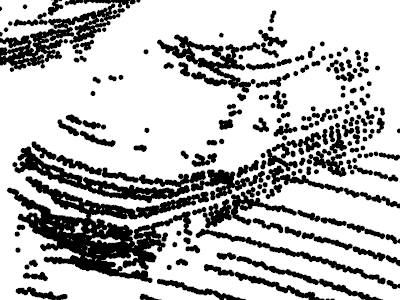
\includegraphics[width=1in]{Graphics/LidarCar0.01.png}
%\caption{fig2}
\end{minipage}%
}%
\subfigure[FGSM with \(\epsilon\) 0.02]{
\begin{minipage}[t]{0.25\linewidth}
\centering
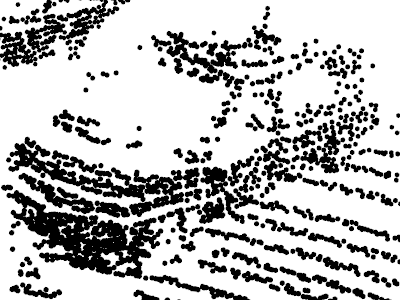
\includegraphics[width=1in]{Graphics/LidarCar0.02.png}
%\caption{fig2}
\end{minipage}
}%
\subfigure[FGSM with \(\epsilon\) 0.04]{
\begin{minipage}[t]{0.25\linewidth}
\centering

\includegraphics[width=1in]{Graphics/LidarCar0.04.png}
%\caption{fig2}
\end{minipage}
}%
\centering
\caption{FGSM with different \(\epsilon\) on Point Clouds, where OPC represents original point clouds and the other three figures is the results after applying FGSM attack with different \(\epsilon\) on original point clouds.}
\label{fig:FGSM Comparison}
\end{figure}

\begin{figure}[!htbp]
\centering
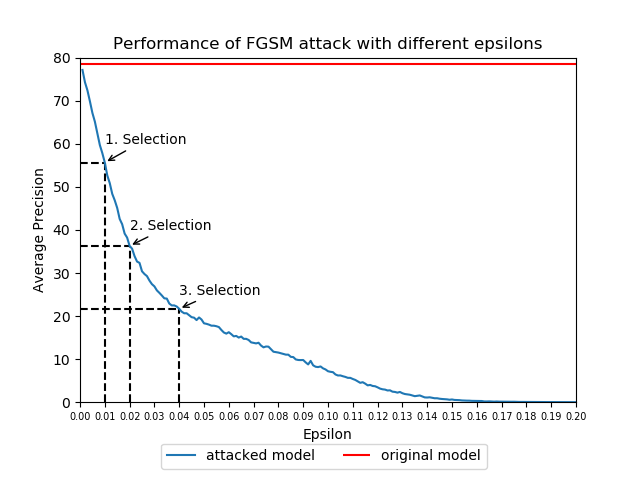
\includegraphics[scale=0.9]{Graphics/Select Epsilons.png}
\caption{Results of FGSM Attack with different Epsilons}
\label{fig:Select Epsilons}
\end{figure}

\subsection{Attack Features}
In Chapter 3 we introduce the features represents different dimensions of LiDAR. In Figure 4.2, when attacking only one feature, we observe x coordinate is the most sensitive. When attacking multiple features, the combination of coordinates \(xyz\) and intensity \(r\) has the most significant performance.
\begin{figure}[!htbp]
\centering
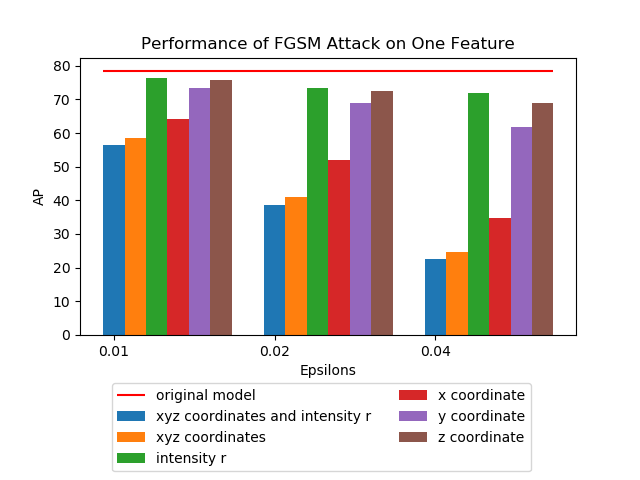
\includegraphics[scale=0.9]{Graphics/Attack Features.png}
\caption{Performance of FGSM Attack on Different Features}
\label{fig:Attack Features}
\end{figure}

% PC Comparison
\begin{figure}[htbp]
\centering

\subfigure[OPC]{
\begin{minipage}[t]{0.25\linewidth}
\centering
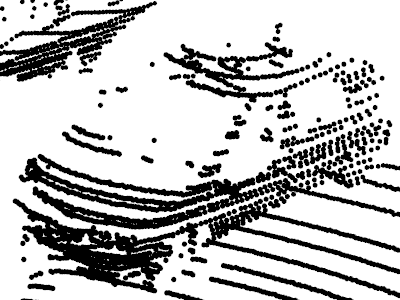
\includegraphics[width=1in]{Graphics/LidarCar0.png}
%\caption{fig1}
\end{minipage}%
}%
\subfigure[Coordinates \(xyz\) with \(\epsilon\) 0.01]{
\begin{minipage}[t]{0.25\linewidth}
\centering
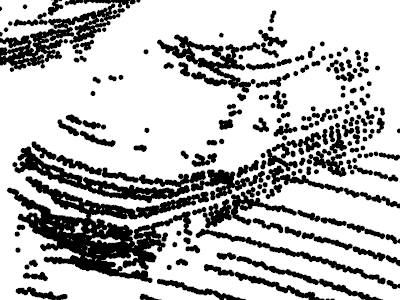
\includegraphics[width=1in]{Graphics/LidarCar0.01.png}
%\caption{fig2}
\end{minipage}%
}%
\subfigure[Coordinates \(xyz\) with \(\epsilon\) 0.02]{
\begin{minipage}[t]{0.25\linewidth}
\centering
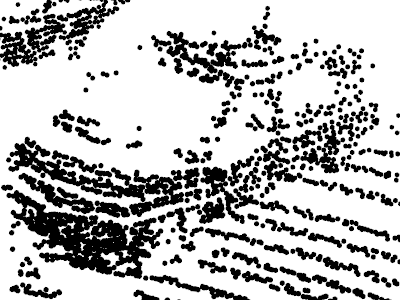
\includegraphics[width=1in]{Graphics/LidarCar0.02.png}
%\caption{fig1}
\end{minipage}%
}%
\subfigure[Coordinates \(xyz\) with \(\epsilon\) 0.04]{
\begin{minipage}[t]{0.25\linewidth}
\centering

\includegraphics[width=1in]{Graphics/LidarCar0.04.png}
%\caption{fig2}
\end{minipage}%
}%

\subfigure[OPC]{
\begin{minipage}[t]{0.25\linewidth}
\centering
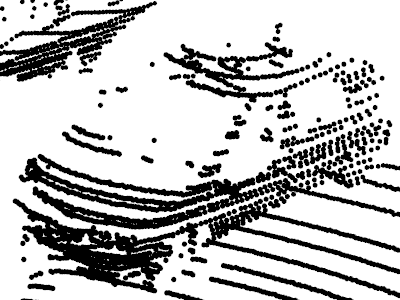
\includegraphics[width=1in]{Graphics/LidarCar0.png}
%\caption{fig2}
\end{minipage}
}%
\subfigure[Coordinate \(x\) with \(\epsilon\) 0.01]{
\begin{minipage}[t]{0.25\linewidth}
\centering
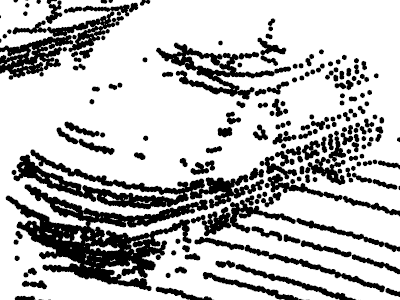
\includegraphics[width=1in]{Graphics/lidar_x_0.01.png}
%\caption{fig2}
\end{minipage}
}%
\subfigure[Coordinate \(x\) with \(\epsilon\) 0.02]{
\begin{minipage}[t]{0.25\linewidth}
\centering
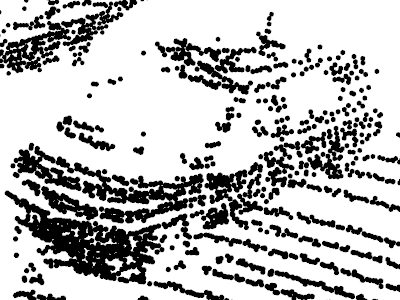
\includegraphics[width=1in]{Graphics/lidar_x_0.02.png}
%\caption{fig2}
\end{minipage}
}%
\subfigure[Coordinate \(x\) with \(\epsilon\) 0.04]{
\begin{minipage}[t]{0.25\linewidth}
\centering

\includegraphics[width=1in]{Graphics/lidar_x_0.04.png}
%\caption{fig2}
\end{minipage}
}%

\subfigure[OPC]{
\begin{minipage}[t]{0.25\linewidth}
\centering
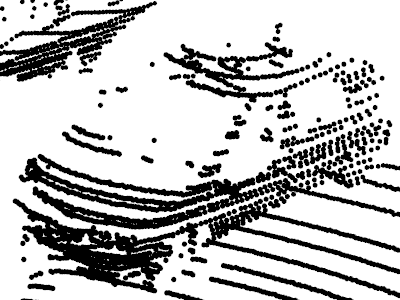
\includegraphics[width=1in]{Graphics/LidarCar0.png}
%\caption{fig2}
\end{minipage}
}%
\subfigure[Coordinate \(y\) with \(\epsilon\) 0.01]{
\begin{minipage}[t]{0.25\linewidth}
\centering
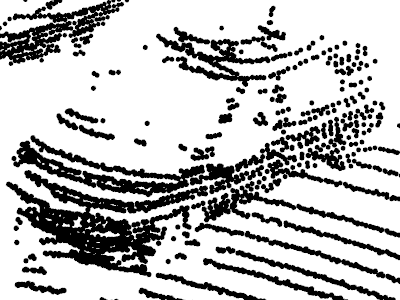
\includegraphics[width=1in]{Graphics/lidar_y_0.01.png}
%\caption{fig2}
\end{minipage}
}%
\subfigure[Coordinate \(y\) with \(\epsilon\) 0.02]{
\begin{minipage}[t]{0.25\linewidth}
\centering
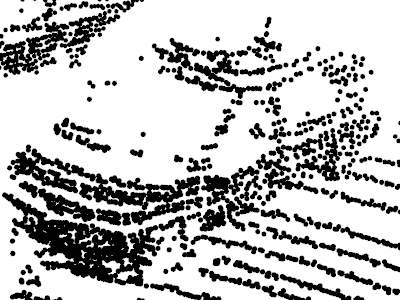
\includegraphics[width=1in]{Graphics/lidar_y_0.02.png}
%\caption{fig2}
\end{minipage}
}%
\subfigure[Coordinate \(y\) with \(\epsilon\) 0.04]{
\begin{minipage}[t]{0.25\linewidth}
\centering
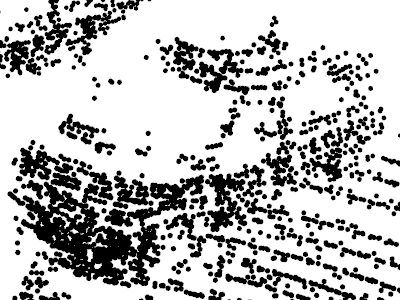
\includegraphics[width=1in]{Graphics/lidar_y_0.04.png}
%\caption{fig2}
\end{minipage}
}%

\subfigure[OPC]{
\begin{minipage}[t]{0.25\linewidth}
\centering
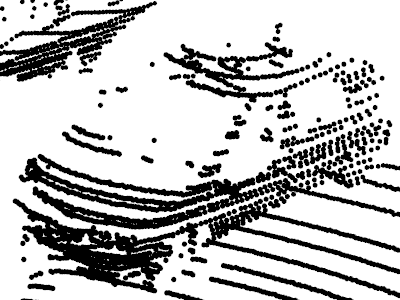
\includegraphics[width=1in]{Graphics/LidarCar0.png}
%\caption{fig2}
\end{minipage}
}%
\subfigure[Coordinate \(z\) with \(\epsilon\) 0.01]{
\begin{minipage}[t]{0.25\linewidth}
\centering
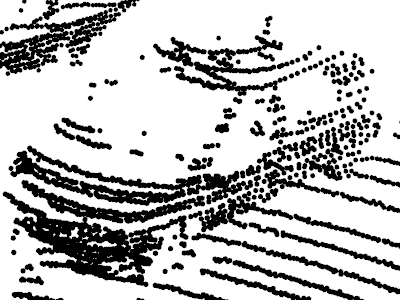
\includegraphics[width=1in]{Graphics/lidar_z_0.01.png}
%\caption{fig2}
\end{minipage}
}%
\subfigure[Coordinate \(z\) with \(\epsilon\) 0.02]{
\begin{minipage}[t]{0.25\linewidth}
\centering
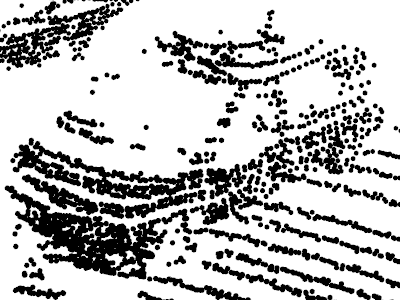
\includegraphics[width=1in]{Graphics/lidar_z_0.02.png}
%\caption{fig2}
\end{minipage}
}%
\subfigure[Coordinate \(z\) with \(\epsilon\) 0.04]{
\begin{minipage}[t]{0.25\linewidth}
\centering
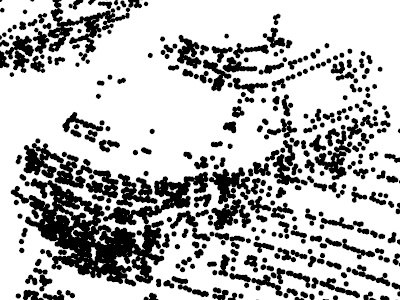
\includegraphics[width=1in]{Graphics/lidar_z_0.04.png}
%\caption{fig2}
\end{minipage}
}%

\centering
\caption{Point Clouds Comparision under 4 Different Features. Where OPC represents original point clouds. the others represents the results after applying different features attack with different \(\epsilon\) on original point clouds. Cause the point cloud visualization with intensity \(r\) is hard to tell, so we only choose 4 features about coordinates: coordinate \(x\), coordinate \(y\), coordinate \(z\), coordinates \(xyz\). }
\label{fig:PC under 4 Features Comparsion}
\end{figure}
\subsection{Adversarial Training}

We use the traditional FGSM adversarial defense method to do the adversarial training. We've introduced, there's other 3 norms (\(L_{1}\),\(L_{2}\),\(L_{2.5}\) to replace \(L_{\infty}\) in FGSM. So we do the adversarial training with 4 different norms and \(\epsilon\) 0.02. And then we got the evaluate result shown in Table \(\ref{tab:FGSM Adversarial Training}\) compare with original model. We've got around 30 models with different evaluation results for each model. We pick the best model based on AP of R40 of 3D bounding boxes of different levels of cars.

FGSM-based Adversarial training is an efficient way to defense adversarial attacks of FGSM. The loss of adversarial training of FGSM:
\begin{center}
          \(Loss_{train} = 1/2*(Loss_{original}+Loss_{perturbation}) \)
\end{center}
 \begin{table}[!htbp]
  \begin{center}
    
    \begin{tabular}{|c|c|c|c|} % <-- Alignments: 1st column left, 2nd middle and 3rd right, with vertical lines in between
      \hline
      \multirow{2}{*}{Models} & \multicolumn{3}{c|}{Average Precision of Different levels of Car}\\
    \cline{2-4}
       &\textbf{Moderate(AP)} & \textbf{(Easy(AP)}& \textbf{Hard(AP)}\\
      \hline
      Original Model & 78.50 & 89.03 & 75.67\\
      \(L_{1}\) Defense Model &  77.83 & 88.26& 74.81\\
      \(L_{2}\) Defense Model & 78.09 & 89.07&75.12\\
      \(L_{2.5}\) Defense Model & 77.75 & 87.41&74.90\\
      \(L_{\infty}\) Defense Model & 76.88 & 87.17&74.22\\
      IFGSM \(L_{2}\) Defense Model & 77.85 & 87.75&75.00\\
    \hline
    \end{tabular}
\caption{Adversarial Training Results Compare with Original Results}
  \end{center}
  \label{tab:FGSM Adversarial Training}
\end{table}

We've found the adversarial defense will not make the model performs better, but could achieve similar 3D AP Scores. But whether the defense model can defense the adversarial attack? We've implemented FGSM attacks with 4 different norm on 5 different models (1 original model and 4 norms defensed models).

\begin{figure}[!htbp]
\centering
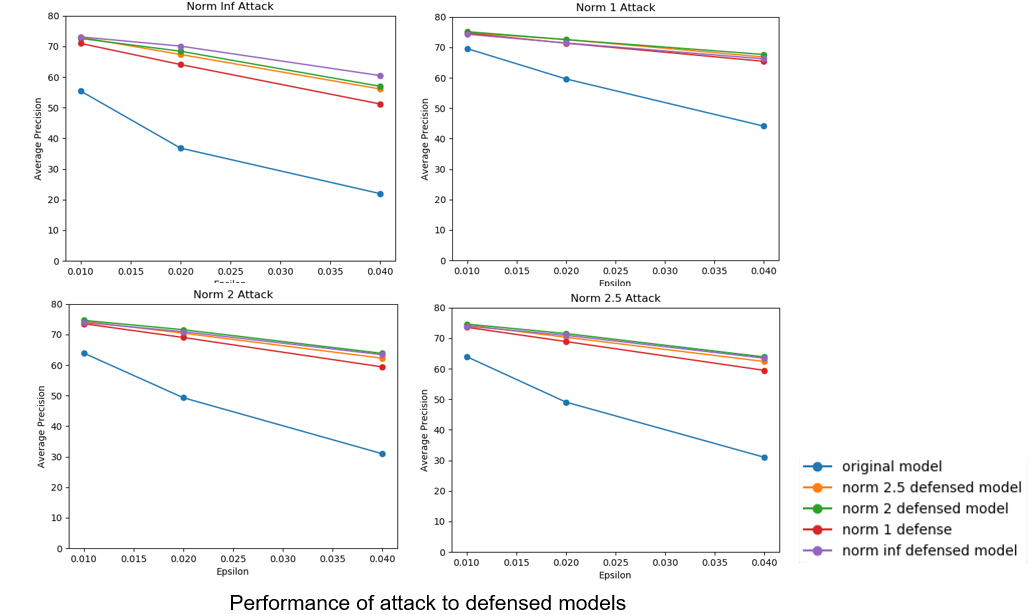
\includegraphics[scale=0.6]{Graphics/Defense Models Attack.png}
\caption{Performance of Attack to Defensed Models}
\label{fig:Defensed Models}
\end{figure}

We've seen the Figure 4.3, the 5 colors of lines represents the AP score from different models. Here are some results we've got from this graph:

1. The attack results of the original model is this blue line. In all these four pictures, this blue line is substantial below other lines, so we conclude FGSM defense models can defend FGSM attack.

2. In the \(L_{\infty}\) attack, the average precision of these five models are smaller than that of other three attacks. So,we know \(L_{\infty}\) attack has the most substantial impact on these five models.

3. In the \(L_{\infty}\) attack, the purple line, which is \(L_{\infty}\) defensed model, is the highest, showing that \(L_{\infty}\) defensed model performs best in the \(L_{\infty}\) attack.

4. The green line is the highest in the these three pictures, indicating that \(L_{2}\) defensed model 
performs best in \(L_{1}\), \(L_{2}\), \(L_{2.5}\) attack. In general, \(L_{2}\) norm defensed model has the best performance.

Considering all these results, we use \(L_{\infty}\) attack and \(L_{2}\) defensed model for the 
next step.

We've also plot the comparison of 4 norms attack under 3 different epsilons on original model, as Figure \(\ref{fig:PC under 4 Noms Comparsion}\) shown. 

% PC Comparison
\begin{figure}[htbp]
\centering

\subfigure[OPC]{
\begin{minipage}[t]{0.25\linewidth}
\centering
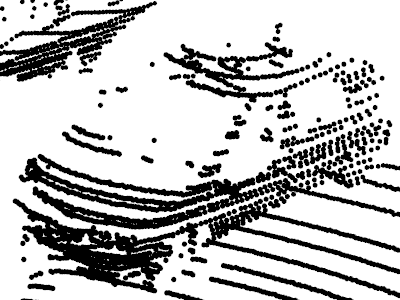
\includegraphics[width=1in]{Graphics/LidarCar0.png}
\end{minipage}%
}%
\subfigure[\(L_{\infty}\) with \(\epsilon\) 0.01]{
\begin{minipage}[t]{0.25\linewidth}
\centering
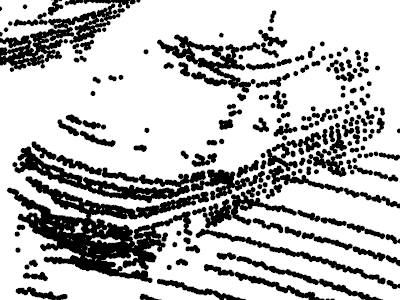
\includegraphics[width=1in]{Graphics/LidarCar0.01.png}
\end{minipage}%
}%
\subfigure[\(L_{\infty}\) with \(\epsilon\) 0.02]{
\begin{minipage}[t]{0.25\linewidth}
\centering
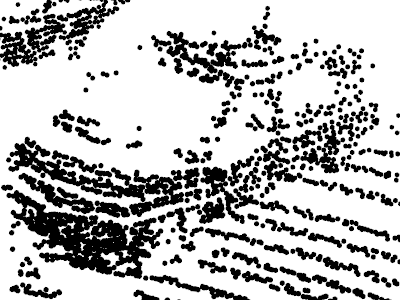
\includegraphics[width=1in]{Graphics/LidarCar0.02.png}
\end{minipage}%
}%
\subfigure[\(L_{\infty}\) with \(\epsilon\) 0.04]{
\begin{minipage}[t]{0.25\linewidth}
\centering

\includegraphics[width=1in]{Graphics/LidarCar0.04.png}
\end{minipage}%
}%

\subfigure[OPC]{
\begin{minipage}[t]{0.25\linewidth}
\centering
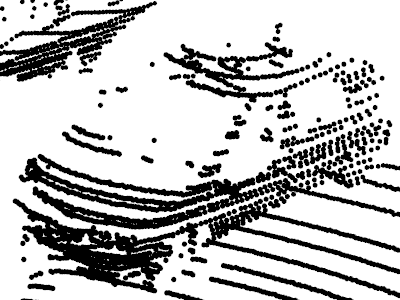
\includegraphics[width=1in]{Graphics/LidarCar0.png}
\end{minipage}
}%
\subfigure[\(L_{1}\) with \(\epsilon\) 0.01]{
\begin{minipage}[t]{0.25\linewidth}
\centering
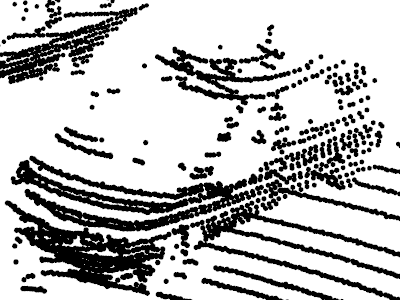
\includegraphics[width=1in]{Graphics/Lidar_1_0.01.png}
\end{minipage}
}%
\subfigure[\(L_{1}\) with \(\epsilon\) 0.02]{
\begin{minipage}[t]{0.25\linewidth}
\centering
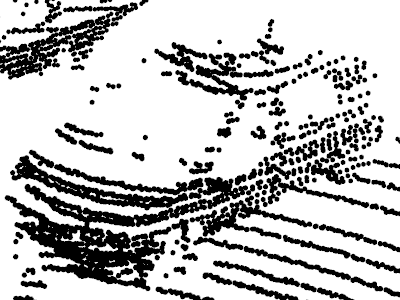
\includegraphics[width=1in]{Graphics/Lidar_1_0.02.png}
\end{minipage}
}%
\subfigure[\(L_{1}\) with \(\epsilon\) 0.04]{
\begin{minipage}[t]{0.25\linewidth}
\centering
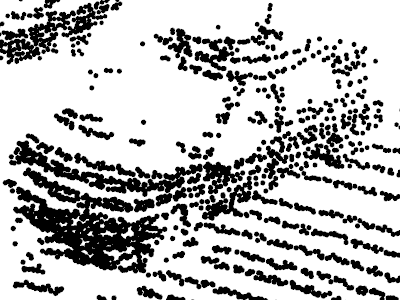
\includegraphics[width=1in]{Graphics/Lidar_1_0.04.png}
\end{minipage}
}%

\subfigure[OPC]{
\begin{minipage}[t]{0.25\linewidth}
\centering
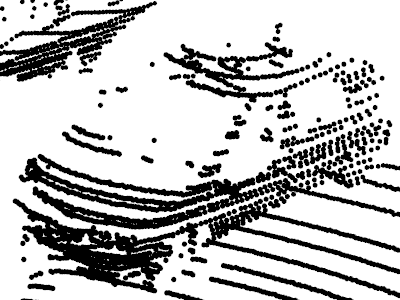
\includegraphics[width=1in]{Graphics/LidarCar0.png}
\end{minipage}
}%
\subfigure[\(L_{2}\) with \(\epsilon\) 0.01]{
\begin{minipage}[t]{0.25\linewidth}
\centering
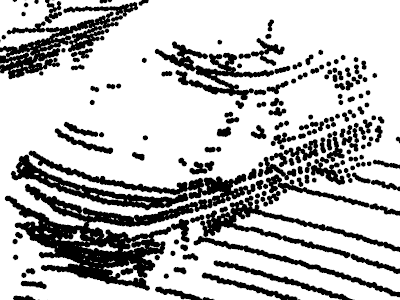
\includegraphics[width=1in]{Graphics/Lidar_2_0.01.png}
\end{minipage}
}%
\subfigure[\(L_{2}\) with \(\epsilon\) 0.02]{
\begin{minipage}[t]{0.25\linewidth}
\centering
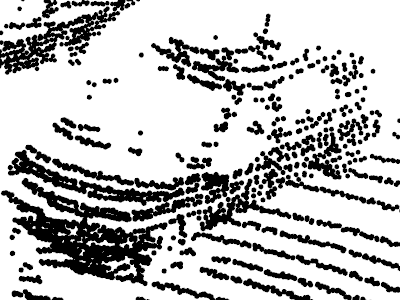
\includegraphics[width=1in]{Graphics/Lidar_2_0.02.png}
\end{minipage}
}%
\subfigure[\(L_{2}\) with \(\epsilon\) 0.04]{
\begin{minipage}[t]{0.25\linewidth}
\centering
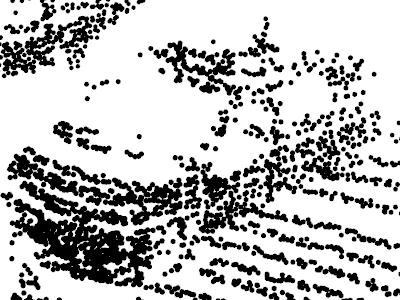
\includegraphics[width=1in]{Graphics/Lidar_2_0.04.png}
\end{minipage}
}%

\subfigure[OPC]{
\begin{minipage}[t]{0.25\linewidth}
\centering
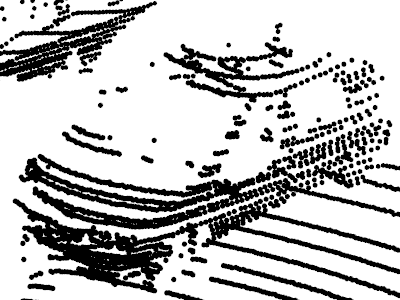
\includegraphics[width=1in]{Graphics/LidarCar0.png}
\end{minipage}
}%
\subfigure[\(L_{2.5}\) with \(\epsilon\) 0.01]{
\begin{minipage}[t]{0.25\linewidth}
\centering
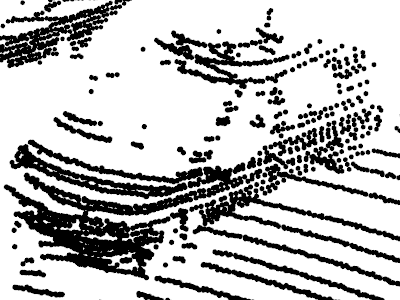
\includegraphics[width=1in]{Graphics/Lidar_2.5_0.01.png}
\end{minipage}
}%
\subfigure[\(L_{\infty}\) with \(\epsilon\) 0.02]{
\begin{minipage}[t]{0.25\linewidth}
\centering
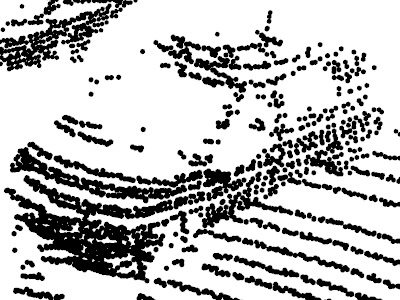
\includegraphics[width=1in]{Graphics/Lidar_2.5_0.02.png}
\end{minipage}
}%
\subfigure[\(L_{2.5}\) with \(\epsilon\) 0.04]{
\begin{minipage}[t]{0.25\linewidth}
\centering
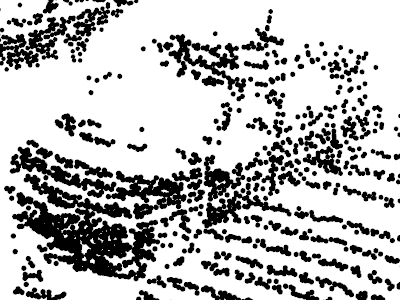
\includegraphics[width=1in]{Graphics/Lidar_2.5_0.04.png}
\end{minipage}
}%

\centering
\caption{Point Clouds Comparision under 4 Norms}
\floatfoot{Where OPC represents original point clouds. the others represents the results after applying FGSM attack with different norm type and \(\epsilon\) on original point clouds }
\label{fig:PC under 4 Noms Comparsion}
\end{figure}


\subsection{FGSM Variants Attack and Defense}
To check whether FGSM defensed model can defense FGSM variants attack, we compare two 
models, the original model, which is non-defensed, and \(L_{2}\) defensed model. The attack 
norm we use here is \(L_{\infty}\). And the results are Figure 4.4.
\begin{figure}[!htbp]
\centering
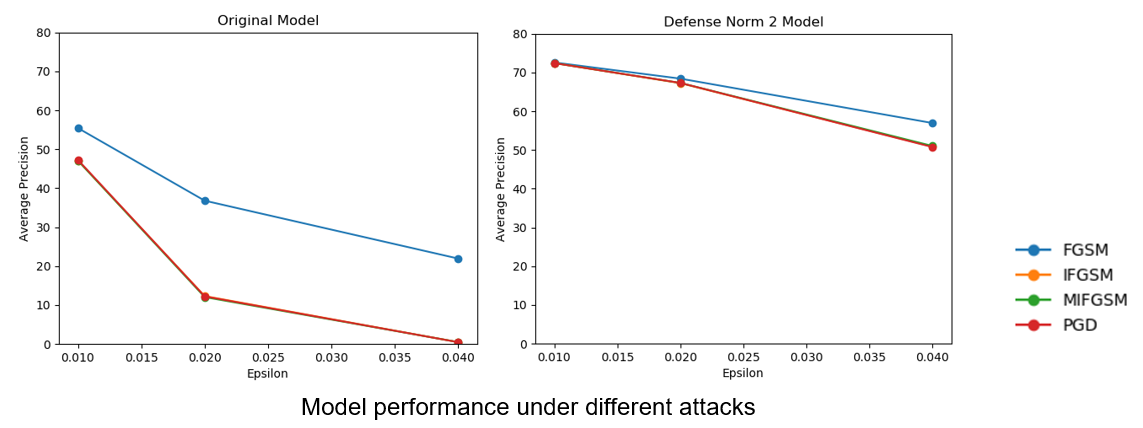
\includegraphics[scale=0.5]{Graphics/FGSM Variants.png}
\caption{Model performance under different attacks}
\label{fig:FGSM Variants}
\end{figure}
% PC Comparison
\begin{figure}[htbp]
\centering

\subfigure[OPC]{
\begin{minipage}[t]{0.25\linewidth}
\centering
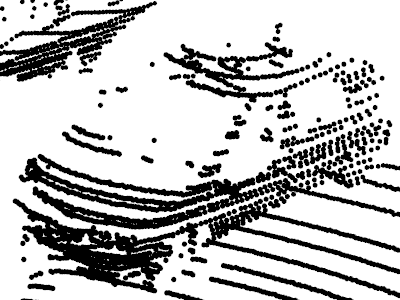
\includegraphics[width=1in]{Graphics/LidarCar0.png}
\end{minipage}%
}%
\subfigure[\(L_{\infty}\) with \(\epsilon\) 0.01]{
\begin{minipage}[t]{0.25\linewidth}
\centering
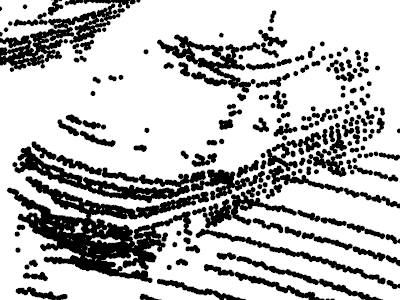
\includegraphics[width=1in]{Graphics/LidarCar0.01.png}
\end{minipage}%
}%
\subfigure[\(L_{\infty}\) with \(\epsilon\) 0.02]{
\begin{minipage}[t]{0.25\linewidth}
\centering
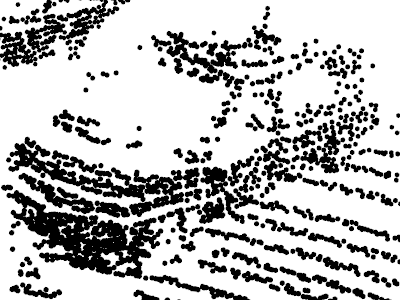
\includegraphics[width=1in]{Graphics/LidarCar0.02.png}
\end{minipage}%
}%
\subfigure[\(L_{\infty}\) with \(\epsilon\) 0.04]{
\begin{minipage}[t]{0.25\linewidth}
\centering

\includegraphics[width=1in]{Graphics/LidarCar0.04.png}
\end{minipage}%
}%

\subfigure[OPC]{
\begin{minipage}[t]{0.25\linewidth}
\centering
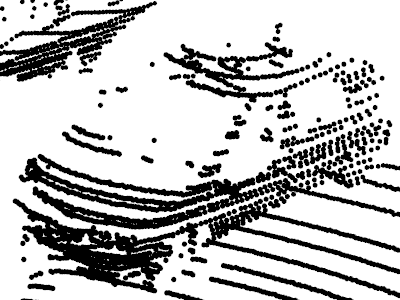
\includegraphics[width=1in]{Graphics/LidarCar0.png}
\end{minipage}
}%
\subfigure[IFGSM with \(\epsilon\) 0.01]{
\begin{minipage}[t]{0.25\linewidth}
\centering
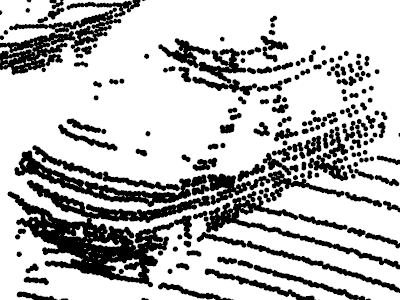
\includegraphics[width=1in]{Graphics/lidar_ifgsm_0.01.png}
\end{minipage}
}%
\subfigure[IFGSM with \(\epsilon\) 0.02]{
\begin{minipage}[t]{0.25\linewidth}
\centering
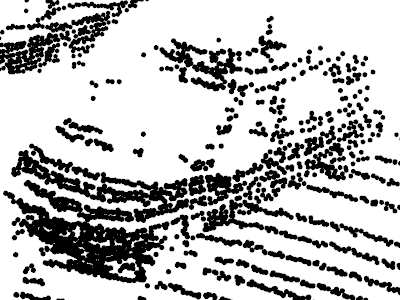
\includegraphics[width=1in]{Graphics/lidar_ifgsm_0.02.png}
\end{minipage}
}%
\subfigure[IFGSM with \(\epsilon\) 0.04]{
\begin{minipage}[t]{0.25\linewidth}
\centering
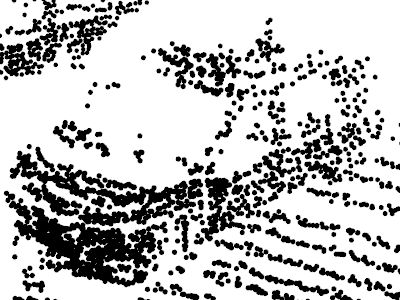
\includegraphics[width=1in]{Graphics/lidar_ifgsm_0.04.png}
\end{minipage}
}%

\subfigure[OPC]{
\begin{minipage}[t]{0.25\linewidth}
\centering
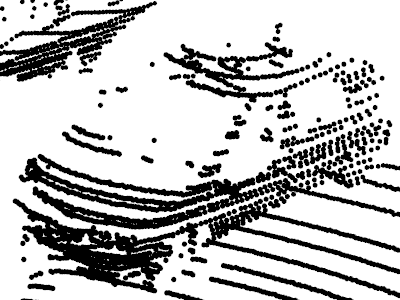
\includegraphics[width=1in]{Graphics/LidarCar0.png}
\end{minipage}
}%
\subfigure[PGD with \(\epsilon\) 0.01]{
\begin{minipage}[t]{0.25\linewidth}
\centering
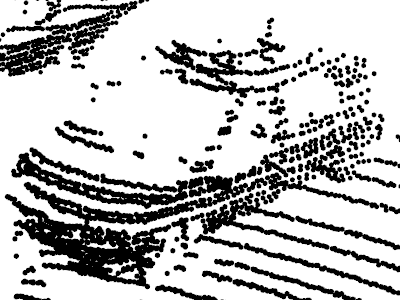
\includegraphics[width=1in]{Graphics/lidar_pgd_0.01.png}
\end{minipage}
}%
\subfigure[PGD with \(\epsilon\) 0.02]{
\begin{minipage}[t]{0.25\linewidth}
\centering
\includegraphics[width=1in]{Graphics/lidar_pgd_0.02.png}
\end{minipage}
}%
\subfigure[PGD with \(\epsilon\) 0.04]{
\begin{minipage}[t]{0.25\linewidth}
\centering
\includegraphics[width=1in]{Graphics/lidar_pgd_0.04.png}
\end{minipage}
}%

\subfigure[OPC]{
\begin{minipage}[t]{0.25\linewidth}
\centering
\includegraphics[width=1in]{Graphics/LidarCar0.png}
\end{minipage}
}%
\subfigure[MIFGSM with \(\epsilon\) 0.01]{
\begin{minipage}[t]{0.25\linewidth}
\centering
\includegraphics[width=1in]{Graphics/lidar_momentum_0.01.png}
\end{minipage}
}%
\subfigure[MIFGSM with \(\epsilon\) 0.02]{
\begin{minipage}[t]{0.25\linewidth}
\centering
\includegraphics[width=1in]{Graphics/lidar_momentum_0.02.png}
\end{minipage}
}%
\subfigure[MIFGSM with \(\epsilon\) 0.04]{
\begin{minipage}[t]{0.25\linewidth}
\centering
\includegraphics[width=1in]{Graphics/lidar_momentum_0.04.png}
\end{minipage}
}%

\centering
\caption{Point Clouds Comparision under 4 FGSM Variants}
\floatfoot{Where OPC represents original point clouds. the others represents the results after applying FGSM attack with different norm type and \(\epsilon\) on original point clouds }
\label{fig:PC under 4 Noms Comparsion}
\end{figure}
As the average precision under each epsilon in the right graph are larger than the left picture, 
which indicates that the defensed model effectively defense FGSM variants. In both graphs, the performance of three FGSM variants are very similar, and the blue line of FGSM attack is distinctly above those lines of its variants, so we conclude FGSM variants perform better than FGSM attack.
\section{Drop Critical Points}
\subsection{Drop Critical Points Attack}
\paragraph{Implementation}
The method we've introduced in concepts part. We've proposed two methods to define critical points with critical features. PointPillars\cite{lang_pointpillars_2019} firstly create pillars using fixed number of points per pillar with point clouds. That means it will insert zero points when the pillar can not contain enough points. When we do the experiments, we've found the point with the most critical features will mostly come from the last virtual point and the point with maximum critical feature will part of come from virtual point. We've made some adjustment to let it only remove the truly point from pillar. And we will remove points with pillars number every iteration. And we drop random point per pillar for the comparison. The drop iterations is 1 to 5.
\begin{figure}[!htbp]
\centering
\includegraphics[scale=0.3]{Graphics/Points Drop.png}
\caption{Performance of Drop Points}
\label{fig:Drop Points}
\end{figure}
\paragraph{Results}
% PC Comparison
\begin{figure}[htbp]
\centering

\subfigure[OPC]{
\begin{minipage}[t]{0.25\linewidth}
\centering
\includegraphics[width=1in]{Graphics/LidarCar0.png}
\end{minipage}%
}%

\subfigure[Drop Critical Point 1 with Iteration 1]{
\begin{minipage}[t]{0.25\linewidth}
\centering
\includegraphics[width=1in]{Graphics/lidar_criticalmaximum_1.png}
\end{minipage}%
}%
\subfigure[Drop Critical Point 2 with Iteration 1]{
\begin{minipage}[t]{0.25\linewidth}
\centering
\includegraphics[width=1in]{Graphics/lidar_criticalmost_1.png}
\end{minipage}%
}%
\subfigure[Drop Random Point with Iteration 1]{
\begin{minipage}[t]{0.25\linewidth}
\centering
\includegraphics[width=1in]{Graphics/lidar_random_1.png}
\end{minipage}%
}%

\subfigure[Drop Critical Point 1 with Iteration 2]{
\begin{minipage}[t]{0.25\linewidth}
\centering
\includegraphics[width=1in]{Graphics/lidar_criticalmaximum_2.png}
\end{minipage}%
}%
\subfigure[Drop Critical Point 2 with Iteration 2]{
\begin{minipage}[t]{0.25\linewidth}
\centering
\includegraphics[width=1in]{Graphics/lidar_criticalmost_2.png}
\end{minipage}%
}%
\subfigure[Drop Random Point with Iteration 2]{
\begin{minipage}[t]{0.25\linewidth}
\centering
\includegraphics[width=1in]{Graphics/lidar_random_2.png}
\end{minipage}%
}%

\subfigure[Drop Critical Point 1 with Iteration 3]{
\begin{minipage}[t]{0.25\linewidth}
\centering
\includegraphics[width=1in]{Graphics/lidar_criticalmaximum_3.png}
\end{minipage}%
}%
\subfigure[Drop Critical Point 2 with Iteration 3]{
\begin{minipage}[t]{0.25\linewidth}
\centering
\includegraphics[width=1in]{Graphics/lidar_criticalmost_3.png}
\end{minipage}%
}%
\subfigure[Drop Random Point with Iteration 3]{
\begin{minipage}[t]{0.25\linewidth}
\centering
\includegraphics[width=1in]{Graphics/lidar_random_3.png}
\end{minipage}%
}%

\subfigure[Drop Critical Point 1 with Iteration 4]{
\begin{minipage}[t]{0.25\linewidth}
\centering
\includegraphics[width=1in]{Graphics/lidar_criticalmaximum_4.png}
\end{minipage}%
}%
\subfigure[Drop Critical Point 2 with Iteration 4]{
\begin{minipage}[t]{0.25\linewidth}
\centering
\includegraphics[width=1in]{Graphics/lidar_criticalmost_4.png}
\end{minipage}%
}%
\subfigure[Drop Random Point with Iteration 4]{
\begin{minipage}[t]{0.25\linewidth}
\centering
\includegraphics[width=1in]{Graphics/lidar_random_4.png}
\end{minipage}%
}%

\subfigure[Drop Critical Point 1 with Iteration 5]{
\begin{minipage}[t]{0.25\linewidth}
\centering
\includegraphics[width=1in]{Graphics/lidar_criticalmaximum_5.png}
\end{minipage}%
}%
\subfigure[Drop Critical Point 2 with Iteration 5]{
\begin{minipage}[t]{0.25\linewidth}
\centering
\includegraphics[width=1in]{Graphics/lidar_criticalmost_5.png}
\end{minipage}%
}%
\subfigure[Drop Random Point with Iteration 5]{
\begin{minipage}[t]{0.25\linewidth}
\centering
\includegraphics[width=1in]{Graphics/lidar_random_5.png}
\end{minipage}%
}%

\centering
\caption{Point Clouds Comparision under 3 Drop Methods}
\floatfoot{Where OPC represents original point clouds. the others represents the results after applying FGSM attack with different norm type and \(\epsilon\) on original point clouds }
\label{fig:PC under 4 Noms Comparsion}
\end{figure}
In the Table 4.4, the green and blue columns are attacks of dropping critical points, and the purple column shows the attack by dropping points randomly. 

(1)The orange column is the highest when dropping different point numbers, so we can say the attack of critical points drop performs more effectively than random points drop.

(2)Since the green column and blue column have roughly similar height, we could say the two methods have similar results. 

\subsection{Drop Critical Points Defense}
Similar to FGSM-based adversarial defense we use the same loss ratio for normal train loss and adversarial loss. But the adversarial loss will get from the point clouds after dropping critical points. But we've tried drop pillar number points for training. Then it will make the moderate AP score drop nearly 15. After training drop less critical points, points of 5\% pillars number to points of 1\% pillars number, which didn't make AP Score performs better. We've also tried with random point drop to defense. And the random drop have two methods:
randomly drop point from each pillar and drop point randomly from point clouds. The comparison result between 4 defensed models and original model is in Table \(\ref{tab:Drop Adversarial Training}\)
 \begin{table}[!htbp]
  \begin{center}
    
    \begin{tabular}{|c|c|c|c|} % <-- Alignments: 1st column left, 2nd middle and 3rd right, with vertical lines in between
      \hline
      \multirow{2}{*}{Models} & \multicolumn{3}{c|}{AP of Different Levels of Car}\\
    \cline{2-4}
       &\textbf{Moderate(AP)} & \textbf{(Easy(AP)}& \textbf{Hard(AP)}\\
      \hline
      Original Model & 78.50 & 89.03 & 75.67\\
      Drop Critical Points Defensed Model 1 & 64.69 & 74.96& 63.11\\
      Drop Critical Points Defensed Model 2 & 65.07 & 75.37& 62.68\\
      Randomly Drop Points Defensed Model 1& 62.71 & 73.05&60.92\\
      Randomly Drop Points Defensed Model 2& 68.52 & 79.51&65.22\\
    \hline
    \end{tabular}
\caption{Adversarial Training Results Compare with Original Results. All defensed Model will drop points with 1\% of pillars numbers, Drop critical points defensed model 1 represents drop critical points with criterion 1, which is the point with most critical features. Drop critical points defensed model 2 represents drop critical points with criterion 2, which is the point with maximum critical value. Randomly drop points defensed model drop the point from pillars and randomly drop points defensed model 2 drop the point from original point.}
  \end{center}
  \label{tab:Drop Adversarial Training}
\end{table}
\subsection{Attack on Defensed Models}
We want to see if defensed models can defense critical drop attacks. We've tested 3 drop methods on 4 defensed models. But the AP scores of trained models is far from original models. So we changed the evaluation metric to relative drop of each models
\section{Points Perturbation and Points Drop}
\subsection{Test Models Robustness}
The last two sections, we've proposed adversarial attack methods based on models. We've also tried to design some adversarial methods not relying on specified model. Then we introduce the Gaussian noise perturbation and drop points randomly to create a benchmark datasets to test more models' robustness.
We've tried to create 20 datasets:

1. We add Gaussian noise perturbation with \(\mu\) 0 \(\sigma\) 0.05, 0.1, 0.15, 0.2, 0.25 to coordinate \(xyz\) of point clouds, then we do the adjustment after perturbation.

2. We add Gaussian noise with \(\mu\) 0 \(\sigma\) 0.15, 0.2, 0.25, 0.25, 0.3 to intensity \(r\) of point clouds. The intensity \(r\) of point clouds in KITTI\cite{geiger_vision_2013} datasets changes from 0 to 0.99. After perturbation of intensity \(r\), we will truncate the values exceed the range. We've found if the \(\sigma\) is smaller than 0.15, the AP score of detection model will not change.

3. We add Gaussian noise to coordinate \(xyz\) and intensity \(r\) with \(\mu\) 0 \(\sigma\) 0.05, 0.1, 0.15, 0.2, 0.25, and will do the adjustment combining method 1 and 2. 

4. We drop random points with the different percent 5\% 10\% 15\% 20\% 25\% of the total number of point clouds. We've found if we drop more than 30\% points of the total number, PointRCNN\cite{shi_pointrcnn_2019} will not work.

We've used the pretrained model in OpenPCDet and there's pretrained model of PointPillar\cite{lang_pointpillars_2019}, PointRCNN, PartA2\cite{shi_points_2020}, Second\cite{yan_second_2018}, PVRCNN\cite{shi_pv-rcnn_2021} trained under KITTI. We've used relative AP Score intorduced in Chapter 3 to test these models' robustness.
\begin{figure}[!htbp]
\centering
\includegraphics[scale=0.3]{Graphics/Relative AP.png}
\caption{Robustness of Detection Models}
\label{fig:Relative AP}
\end{figure}

In Figure 4.6, the vertical axis is the relative performance under perturbation, the highest column is PointRCNN, so we know it performs best. The performance of other detection models are 
almost the same.

The changes of \(\sigma\) equals to 0.25 to point cloud is actually huge, there's 68\% of perturbation less than 0.25, but 27\% of perturbation between 0.25 to 0.5 and 0.5 means 0.5 meter perturbation to a point. The perturbation is clearly. If we control the \(\sigma\) changes from 0.02 to 0.1 in each methods. Then we've got the relative performances are almost the same as Figure 4.7 shown.
\begin{figure}[!htbp]
\centering
\includegraphics[scale=0.4]{Graphics/Relative AP1.png}
\caption{Robustness of Detection Models}
\label{fig:Relative AP1}
\end{figure}

\subsection{Adversarial Training of Benchmark Datasets}
The datasets is not changed with the different parameters of model. So we've stored the 20 benchmark datasets and merge 20 datasets and original one into a huge dataset for training. PointPillars as the highest training speed in OpenPCDet is trained under the compound datasets to see if the benchmark datasets help detection model performs better. 

 \begin{table}[!htbp]
  \begin{center}
    
    \begin{tabular}{|c|c|c|c|} % <-- Alignments: 1st column left, 2nd middle and 3rd right, with vertical lines in between
      \hline
      \multirow{2}{*}{Models} & \multicolumn{3}{c|}{AP of Different Levels of Car}\\
    \cline{2-4}
       &\textbf{Moderate(AP)} & \textbf{(Easy(AP)}& \textbf{Hard(AP)}\\
      \hline
      Original Model & 78.50 & 89.03 & 75.67\\
      Defensed Model & 75.89 & 87.54&  73.01\\
    \hline
    \end{tabular}
\caption{PointPillars Adversarial Training on Benchmark Datasets and Original KITTI}
  \end{center}
  \label{tab:Benchmark Adversarial Training}
\end{table}
From the comparison of the results of models. Defense Model performs clearly not good as original model.
For the robustness of defensed model of PointPillars. It shows
 \begin{table}[!htbp]
  \begin{center}
    
    \begin{tabular}{|c|c|c|} % <-- Alignments: 1st column left, 2nd middle and 3rd right, with vertical lines in between
      \hline
      \multirow{2}{*}{Models} &\multicolumn{2}{c|}{Robustness of Different Datasets}\\
    \cline{2-3}
      &\textbf{Datasets1(rPP)}&\textbf{Datasets2(rPP)}\\
      \hline
      Original Model&0.76&0.93\\
      Defensed Model&0.88&0.93\\
    \hline
    \end{tabular}
\caption{Robustness on Benchmark Datasets of 2 PointPillars Models}
  \end{center}
  \label{tab:robustness pointpillar}
\end{table}
\section{Adverse Weather Point Clouds Simulation}
The objective is using point clouds under clean weather to simulate point clouds under adverse weather.

We've proposed three simulating methods:

1. Add Gaussian noise perturbation to point clouds under clean weather to simulate.

2. Drop point clouds under clean weather randomly to simulate.

3. Use RANSAC\cite{fischler_random_1981} to get ground plane point clouds cluster, and use DBSCAN\cite{rehman_dbscan_2014} to get the other point clouds parts' clusters as different objects(cars, trees, pedestrian, etc.). We randomly select some points in each cluster and add Gaussian noise perturbation to these points and add these points to original points.

It's hard for naked eyes to tell, which point clouds belong to which weather. We've found there's more precise way, weather point segment network to replace weather classification network. With a better semantic segmentation network Cylinder3D\cite{zhu_cylindrical_2020} trained on DENSE\cite{DENSE}, which performs better than WeatherNet (Table \(\ref{tab:DENSE}\)). So we use Cylinder3D as our evluation network.

 \begin{table}[h!]
  \begin{center}

    \begin{tabular}{|c|c|c|} % <-- Alignments: 1st column left, 2nd middle and 3rd right, with vertical lines in between
      \hline
      \multirow{2}{*}{Methods} & \multicolumn{2}{c|}{Weather Class}\\
    \cline{2-3}
       &\textbf{Clean Points Number} & \textbf{Rain Points Number)}\\
      \hline
      clean Point Clouds(cPC) & 9360 & 11\\
      \hline
      cPC + \(\sigma\) 0.01 perturbation & 6577 & 194\\
      \hline
      cPC + \(\sigma\) 0.05 perturbation & 7600 & 1069\\
      \hline
      cPC + \(\sigma\) 0.1 perturbation & 8142 & 2013\\
      \hline
      cPC + \(\sigma\) 0.2 perturbation & 7857 & 2455\\
      \hline
      cPC + \(\sigma\) 0.3 perturbation & 5659 & 5545\\
      \hline
      Rain Point Cloud & 4129 & 3624\\
    \hline
    \end{tabular}
    \caption{Add Gaussian Noise Perturbation Results}
  \end{center}
    \label{tab:Gaussian Noise Simulate}
\end{table}
In Table \(\ref{tab:Gaussian Noise Simulate}\), we have one clean point clouds(cPC), which aims to simulate rain point cloud with Gaussian noise perturbation. We use Cylinder3D to get the different number of rain and clean point clouds. If the ratio of rain and clean point clouds of the simulated point clouds and rain point clouds are the same, we assume we made a success simulation under evaluation. In the table we've seen when \(\sigma\) equals to 0.3, the ratio is almost the same. Then we think the simulation is success.